\documentclass{article}
\usepackage{float}
\usepackage{amsmath}
\usepackage{hyperref}
\usepackage{xcolor}
\usepackage{algpseudocode}
\usepackage{algorithm}
\usepackage{amssymb}
\usepackage{caption}
\usepackage{subcaption}
\usepackage[margin=1in, top=0.5in]{geometry} 
\usepackage{graphicx} % Required for inserting images

\title{Jane Street Puzzle July 2026}
\author{Andrew Ely}
\date{}

\begin{document}
\maketitle

\begin{figure}[H]
    \centering
    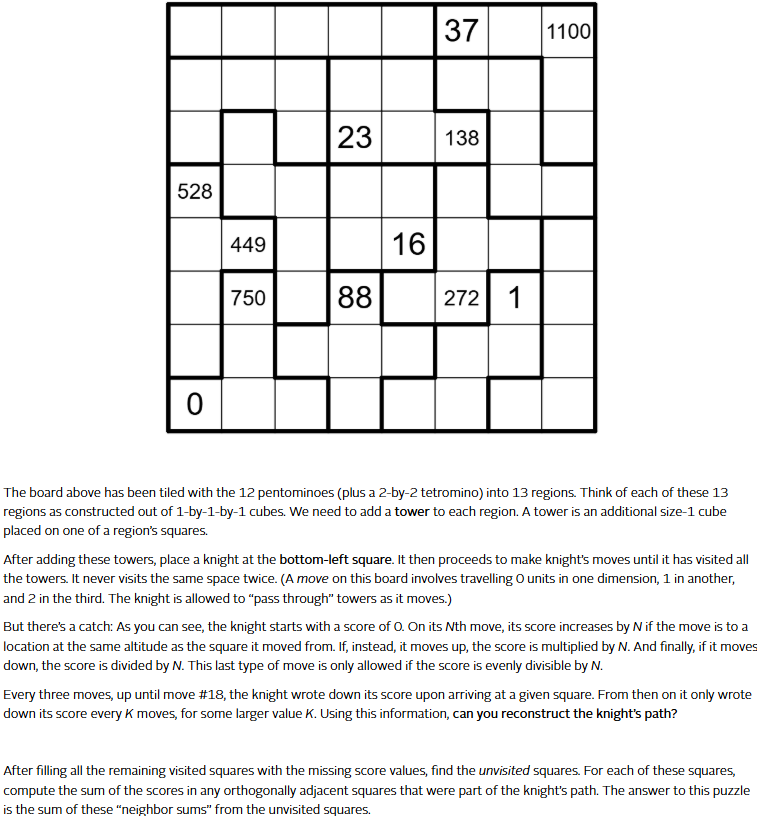
\includegraphics[width=1\linewidth]{img.png}
\end{figure}


\section{Understanding the Problem}

Before attempting to develop a solution to the problem, it is important to understand what the problem at hand is. We are presented with 5 paragraphs in the instructions, and each paragraph provides information about the puzzle. We can break down the information in each paragraph as follows.

\subsection{The boards construction}

The \textcolor{blue}{\href{https://en.wikipedia.org/wiki/Pentomino}{12 pentominos}} refers to the 12 distinct shapes constructed by arranging 1 by 1 equal sized squares without rotation and reflection, and the 2 by 2 tetromino refers to the center square region (where the number 16 is). The instructions mention adding 1 tower to each region, and these towers are size-1 cubes. Notice that there can be at most one tower on a square, so there is only two levels of altitude. A normal 2D chess board is 8 by 8 squres, resulting in 64 discrete spaces for a piece to move to. Adding the towers seems to add an additional dimension, consiting of two levels. However, our board does not really become a 8x8x2 discrete metric space because any assignment of towers to the board results in exactly 64 possible spaces the knight can move. For this reason, it can be helpful to think of our board as simply a 8x8 2D board with the possible attribute of a tower existing in any given cell, which affects the knights movement as follows.

\subsection{How the knight moves}

In standard chess, the knight moves two squares in one direction, and one square in the other direction like the shape of an "L". If we consider a normal chess board with dimensions left/right and up/down, a knight has 2 options of which dimension to move 2 spaces in. Then, we chose which direction for each dimension to move, resulting in the 8 possible moves for a knight to make, not considering moves that are out of the boundaries of the board. Following this same construction, by adding a third dimension to the movement, we have 3 choices for which dimension to move 2 spaces in, and for each of the 3 choices we have 2 choices for which dimension to move 1 space in, while the final dimension follows with 0 spaces. However, we must realize that we cannot move 2 spaces in the up / down dimension because we are only to place one tower on each region, there is no possible way to move 2 units up or down. Then we result with only 4 possible ways to decide what dimensions we will move 2,1, and 0 spaces in. For each of these 4 ways, we have 2 choices for if we should move positive or negative for each of the dimensions we assigned 2 and 1 space movement to. This results in 16 possible movements a knight can make at any given time, without consdering towers/numbers/boundaries. Also notice that the only way for the knight to make any type of move is as follows: normal chess moves must be from either no tower square to no tower square or tower square to tower square, jumping down moves must be from tower square to non tower square, and jumping up moves must be from no tower square to tower square. 

\begin{figure}[H]
\centering
\begin{minipage}{.24\textwidth}
  \centering
  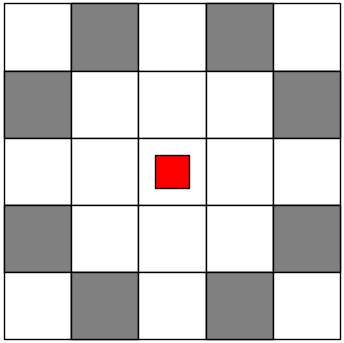
\includegraphics[width=.95\linewidth]{Figure_1.png}
  \caption*{Normal Moves}

\end{minipage}%
\begin{minipage}{.24\textwidth}
  \centering
  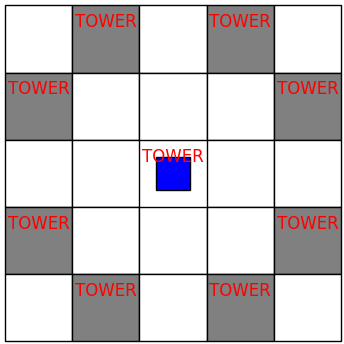
\includegraphics[width=.95\linewidth]{Figure_2.png}
  \caption*{Normal Tower Moves}

\end{minipage}
\begin{minipage}{.24\textwidth}
  \centering
  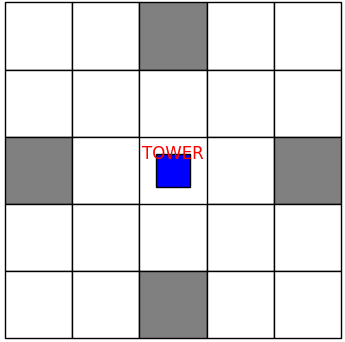
\includegraphics[width=.95\linewidth]{Figure_3.png}
  \caption*{Jump Down Moves}

\end{minipage}
\begin{minipage}{.24\textwidth}
  \centering
  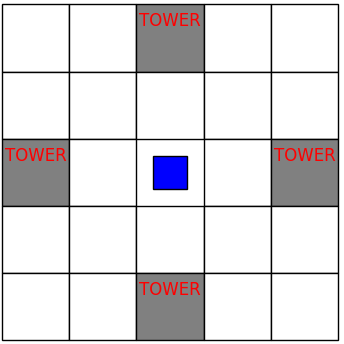
\includegraphics[width=.95\linewidth]{Figure_4.png}
  \caption*{Jump Up Moves}

\end{minipage}
\end{figure}



\subsection{How the score accumulates}

The knight begins at the bottom left square marked with the number 0, awaiting to make the first (N=1) move. If at any move the knight makes a normal move as depicted above, the score accumales by N. If the knight jumps up to a tower, the score is multiplied by N, and if the knight jumps down the score is divided by N which is only allowed if the resulting division is an integer. This divison rule restricts how often this move is available. 

\subsection{The marked numbers}

The numbers represent where the knight marked down its score. There are 12 squares with numbers, and for the first 18 moves the knight marked down every 3 moves. We also start on move 0 on the numbered square 0. This means 7 of the 12 numbered squares will be explored after the first 18 moves. This is critical because after the first 18 moves, the space between when the knight records the number changes.

\subsection{Constructing the final sum}

After recovering the knights path, computing the final sum is straightforward.

\section{Solving the problem}

After fully understanding the problem, we can begin brainstorming an approach for solving. One realization is that for any given location, the knight has at most 8 possible spots it can move to. With every 3 moves requiring the knight to be on a numbered cell for the first 18 moves, the search space for exploring possible paths may actually be quite small. As it turns out, simply evaluating where the knight can move to at each move and ruling out impossible paths is a feasible approach.

We perform a depth-first search over partial knight paths. At each step, it generates every move consistent with the knight’s geometry, the current tower height, and the arithmetic rule associated with the move. It then prunes any path that revisits a cell, places multiple towers in one region, or conflicts with a required numbered cell. The search is divided after move 18 because the spacing of the numbered clues changes at that point. A path is accepted once it visits every numbered cell and places exactly one tower in every region. The psuedo code below provides the alogrithm used to solve the problem.





\subsection{Checking possible moves}


\begin{algorithm}[H]
\caption{Generate possible moves}
\begin{algorithmic}

\Function{GetPossibleMoves}{currentCell,currentMoves}

\State $currentScore \gets currentCell.num$
\State $currentMoveNumber \gets length(currentMoves)$
\State $possibleMoves \gets [\ ]$

\State $moveDirections \gets [$
\Statex $\qquad (2,1,0),(-2,1,0),(2,-1,0),(-2,-1,0),$
\Statex $\qquad (1,2,0),(-1,2,0),(1,-2,0),(-1,-2,0),$
\Statex $\qquad (0,2,1),(0,-2,1),(2,0,1),(-2,0,1),$
\Statex $\qquad (0,2,-1),(0,-2,-1),(2,0,-1),(-2,0,-1)\ ]$

\

\For{move in moveDirections}

    \State $nextRow \gets currentCell.row + move[0]$
    \State $nextCol \gets currentCell.col + move[1]$
    \State $heightChange \gets move[2]$

    \If{$nextRow < 0$ or $nextRow > 7$ or
        $nextCol < 0$ or $nextCol > 7$}
        \State \textbf{continue}
    \EndIf

    \State $nextCell \gets board[nextRow][nextCol]$

    \If{$nextCell.tower \neq None$}
        \State \textbf{continue}
    \EndIf

    \

    \If{$heightChange == 0$}
        \Comment{Normal knight move}

        \State $newScore \gets currentScore + currentMoveNumber$
        \State $newTowerStatus \gets currentCell.tower$

    \ElsIf{$currentCell.tower == True$ and $heightChange == -1$}
        \Comment{Move downward from a tower}

        \If{$currentScore \bmod currentMoveNumber \neq 0$}
            \State \textbf{continue}
        \EndIf

        \State $newScore \gets currentScore/currentMoveNumber$
        \State $newTowerStatus \gets False$

    \ElsIf{$currentCell.tower == False$ and $heightChange == 1$}
        \Comment{Move upward onto a tower}

        \State $newScore \gets currentScore \cdot currentMoveNumber$
        \State $newTowerStatus \gets True$

    \Else
        \State \textbf{continue}
    \EndIf

    \

    \If{$nextCell.num == None$ or $nextCell.num == newScore$}

        \State $newMove.row \gets nextRow$
        \State $newMove.col \gets nextCol$
        \State $newMove.num \gets newScore$
        \State $newMove.tower \gets newTowerStatus$
        \State $newMove.region \gets nextCell.region$

        \State $possibleMoves.append(newMove)$

    \EndIf

\EndFor

\State \Return $possibleMoves$

\EndFunction

\end{algorithmic}
\end{algorithm}


% \subsection{Helper functions for validating a move}

% \begin{algorithm}[H]
% \caption{Construct a sequence of moves}
% \begin{algorithmic}

% \Function{CheckMove}{newMove,currentMoves}

% \State$exploredCells \gets [ \ ]$
% \For{m in currentMoves}
%     \State{exploredCells.append((m.row,m.col))}
% \If{(newMove.row,newMove.col) in exploredCells}
%     \State \Return False
% \EndIf
% \EndFor

% \

% \State$regionsWithTowers \gets [ \ ]$
% \For{m in currentMoves}
% \If{m.tower}
% \State regionsWithTowers.append(m.region)
% \EndIf
% \EndFor

% \If{newMove.tower and newMove.region in regionsWithTowers}
% \State \Return False
% \EndIf

% \

% \State$modulo \gets \text{If first 18 moves then 3, else <k>}$
% \State$moveCountOffset \gets \text{If first 18 moves then 18, else 0}$
% \If{len(currentMoves)-moveCountOffset) \% modulo == 0}
% \If{board[newMove.row][newMove.col].num == newMove.num}
% \State \Return True
% \Else
% \State \Return False
% \EndIf
% \EndIf

% \

% \State \Return True
% \EndFunction

% \end{algorithmic}
% \end{algorithm}






\subsection{Constructing the moves}

\begin{algorithm}[H]
\caption{Construct a sequence of moves}
\begin{algorithmic}
\State$trackedMoves \gets \text{[[\{'row': 7, 'col': 0, 'num': 0, 'tower':  True, 'region': 't'\}],}$
\State$\qquad\qquad\qquad\qquad\text{[\{'row': 7, 'col': 0, 'num': 0, 'tower': False, 'region': 't'\}],]}$

\State$first18moves \gets [ \ ]$

\Function{GetFirst18Moves}{}
\While{trackedMoves}
\State $currentMoves \gets trackedMoves.pop()$
\State $currentCell \gets currentMoves.LastElement()$
\State $possibleMoves \gets \textbf{getPossibleMoves}(currentCell,currentMoves)$
\For{p in possibleMoves}
\If{CheckMove(p,currentMoves)}
\State $ newMoves \gets currentMoves.copy()$
\State $ newMoves.append(p)$
\State $ trackedMoves.append(newMoves)$
\EndIf
\EndFor
\If{length(currentMoves) == 19}
\State$first18moves.append(currentMoves)$ \Comment{We reached a sequence of 18 moves.}
\EndIf
\EndWhile
\EndFunction

\

\Function{GetRestOfMoves}{first18moves}
\State$count \gets 0 $
\For{k in range(4,10)} \Comment{****WE CANT HAVE K > 9****}
\State$trackedMoves \gets first18Moves.copy()$
\While{trackedMoves}
\State $currentMoves \gets trackedMoves.pop()$
\State $currentCell \gets currentMoves.LastElement()$
\State $possibleMoves \gets \textbf{getPossibleMoves}(currentCell,currentMoves)$
\For{p in possibleMoves}
\If{CheckMove(p,currentMoves)}
\State $ newMoves \gets currentMoves.copy()$
\State $ newMoves.append(p)$
\State $ trackedMoves.append(newMoves)$
\If{CheckFinished(newMoves)}
\State \Return newMoves
\EndIf
\EndIf
\EndFor
\If{length(currentMoves) == 19}
\State$first18moves.append(currentMoves)$ \Comment{We reached a sequence of 18 moves.}
\EndIf
\EndWhile
\EndFor
\EndFunction


\end{algorithmic}
\end{algorithm}






% \subsection{Verifying a solution}

% \begin{algorithm}[H]
% \caption{Check if a list of moves is valid}
% \begin{algorithmic}
% \Function{Verify}{moves}
% \State $explored \gets [ \ ]$
% \State $numberedCells \gets \text{List of (x,y) squares with numbers in original board.}$
% \State $regionsWithTowers \gets [ \ ]$
% \State $regions \gets \text{List of regions id's (e.g. chars f,i,l,n,p,..)}$
% \For{m in currentMoves}

% explored.append((m['row'],m['col']))

% \For{n in numberedCells}
% \If{n not in explored} 
%     \State return False 
% \EndIf

% \For{m in moves}
% \If{m.tower and m.region not in regionsWithTowers}
% \State regionsWithTowers.append(m.region)
% \EndIf
% \EndFor

% \For{r in regions}
% \If{r not in regionsWithTowers}
% \State return False
% \EndIf
% \EndFor

% \State return True \Comment{we checked all fail points, this move set is valid, return true.}

% \EndFor
% \EndFor
% \EndFunction
% \end{algorithmic}
% \end{algorithm}






% \subsection{Extracting the final answer}

% \begin{algorithm}[H]
% \caption{Calculate Final Sum}
% \begin{algorithmic}

% \State $solution \gets \text{set of verified moves}$
% \State $directions \gets [(0,1),(0,-1),(-1,0),(1,0)]$
% \State $finalSum \gets 0$
% \State $visited \gets \text{list of squares that the knight explored}$

% \For{i in range(1...8)}
% \For{j in range(1...8)}
% \If{ (i,j) not in visited}
% \For{d in directions}
% \State $neighbor = (i+d[0],j+d[1])$
% \If{neighbor in visited}
% \State $finalSum += neighbor.number$
% \EndIf
% \EndFor
% \EndIf
% \EndFor
% \EndFor

% \State \Return $finalSum$

% \end{algorithmic}
% \end{algorithm}







\end{document}
